\documentclass[spanish]{udpreport}
\usepackage[utf8]{inputenc}
\usepackage[spanish]{babel}

% Podemos establecer el logo de alguna entidad o dejar el de la UDP (defecto)
%\setlogo{EITFI}

\title{Informe Laboratorio III \\ Redes de Datos}
\author{Arturo Mantinetti \\ Manuel Tobar \\ Diego Vilches \\ Nicolas Henriquez}
\email{arturo.mantinetti@mail.udp.cl \\ manuel.tobar@mail.udp.cl
	\\ diego.vilches@mail.udp.cl \\ nicolas.henriquez@mail.udp.cl}
	
\profesor{Profesor \\ Jaime Álvarez}
\ayudante{Ayudante \\ Maximiliano Vega}


\date{10 de Abril de 2016} %Cambie la fecha de 8 a 10 no se si importe (?) - Manuel

% Además podemos establecer la facultad y escuela
% los valores por defecto son los siguientes:
%\udpschool{Escuela de Informática y Telecomunicaciones}
%\udpfaculty{Facultad de Ingeniería}
%\udpuniversity{Universidad Diego Portales}

\begin{document}
\maketitle

\tableofcontents

\chapter{Introducción}

%metanle caca cabros atte. diego
%corrijan mi caca
%recuerden que siempre se habla en tercera persona
%saludos
Este laboratorio consistió en crear paquetes de datos con diferentes parámetros para luego enviarlos por la red, con el fin lo lograr comprender como se conforman y comportan estos según sus características. Esto es posible gracias a un programa llamado 'Scapy' que nos da esas funcionalidades. 

Los paquetes, en este experimento, varían principalmente en la dirección MAC, lo que hace que sean recibidos por distintos equipos. Para esto se ocupa 'Wireshark', programa con el que se puede capturar los paquetes enviados por la red.  Una vez creados y enviados los paquetes a través del Switch, se repite el procedimiento, sólo que esta vez los equipos están conectados a un Hub. 

%Ahi modifique un poco la mierda, pero falta agregar. atte: Manuel


\chapter{Contenido}

\section{Creación de Paquetes}
Para crear un paquete con Scapy, este se tiene que ejecutar vía la consola el siguiente comando:
%Alguna forma bonita de mostrar el comando - Manuel
\\


Este comando iniciara el programa donde se podrá usar sus funciones para la creación de los paquetes. Estos se crean en base a las capas del modelo OSI, sin necesidad de seguir un orden especifico al crear las capas, las cuales el programa permite su uso desde la Capa 2 hasta la que se necesite para el paquete.

\begin{center}
	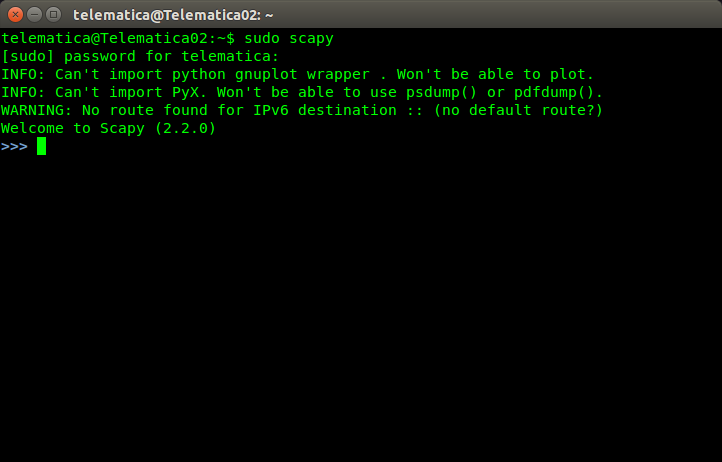
\includegraphics[scale=.37]{imagenes/Scapy_Init.png}
\end{center}

Iniciando con la Capa 2 esta el comando Ether(), este comando permite modificar los parámetros del enlace de datos, en especial las MACs de destino y origen, en este laboratorio se utiliza en demasía esta capa.

%Imagen de los parametros del comando? - Manuel

El siguiente comando, el cual se encarga de la Capa 3, es IP() el cual se encarga de los parámetros de enrutamiento incluyendo protocolos y direcciones lógicas del sistema, las direcciones de IP de origen y destino.

%Imagen de los parametros del comando? - Manuel

%no se que mierda poner para ICMP() - Manuel

%[...] = alguna forma de continuacion del parrafo anterior
[...] ultimo comando a usar, el cual se encarga de la información a enviar, es Raw() este se tiene un String como parámetro para el envío de información a ser usada por el equipo de destino.
%Imagen de los parametros del comando? - Manuel
\\

Una vez creado las capas a usar, con las capas que se estimen convenientes, estas son apiladas en orden ascendente separadas con un '/' para que estas formen un solo paquete que luego puede ser enviado, para el envío del paquete se utiliza el comando sendp() %el cual hace el envio??? - Manuel

%Agregen mucha mierda! - Manuel

\newpage

\section{Switch}

\subsection{Envío de un paquete de datos a FF:FF:FF:FF:FF:FF}
%escribire en primera persona porque me da paja hacerlo en tercera - Manuel
Creamos el paquete con la dirección MAC 'FF:FF:FF:FF:FF:FF' ...

\begin{center}
	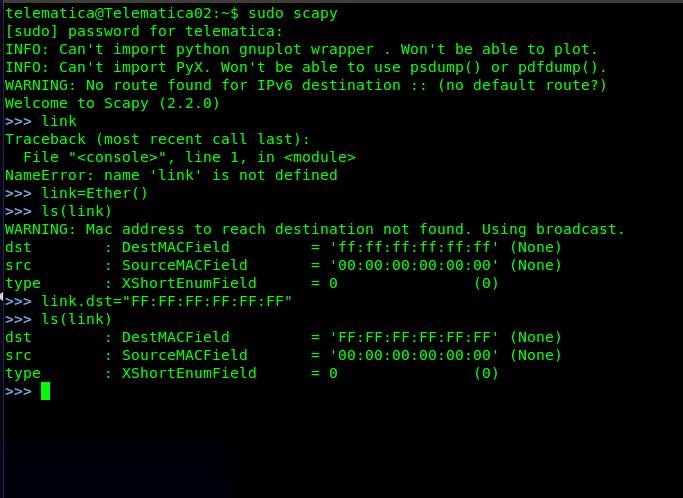
\includegraphics[scale=.37]{imagenes/Switch/Test_1a_b.png}
\end{center}

Al no necesitar ningún parámetro extra en las capas superiores solo las definimos/instanciamos , aunque esto no es necesario para el funcionamiento del paquete (?). Solo modificamos el parámetro de la función Raw() para poder identificar el paquete que nosotros enviamos, una vez hecha la modificación a ese parámetro apilamos el paquete y procedemos el envío de este.

\begin{center}
	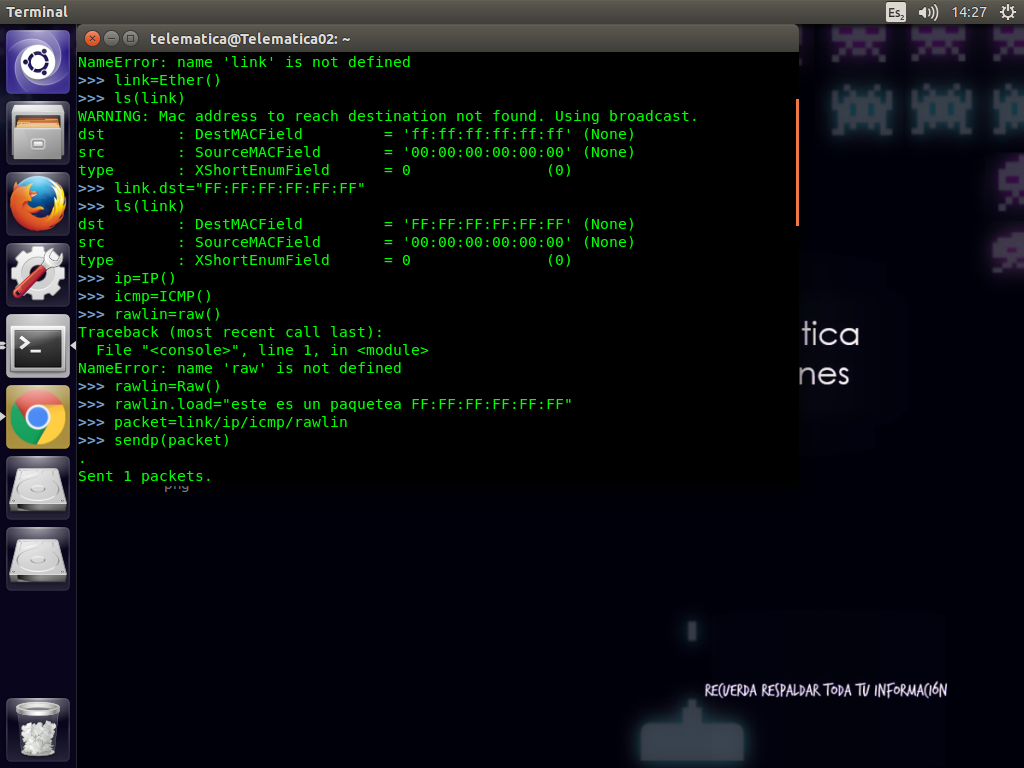
\includegraphics[scale=.37]{imagenes/Switch/Test_1b.png}
\end{center} 

%No hay imagen de wireshark del experimento 1 ... - Manuel

% Al ser la dirección MAC 'FF:FF:FF:FF:FF:FF' la dirección de Broadcast el paquete es enviado a todos los equipos dentro de la red... %Creo que va en cuestionario esta wea...

%agregar mierda Manuel

\subsection{Envío de un paquete de datos con MAC especifica}

Para este segundo experimento, esta vez usamos la siguiente dirección MAC '18:a9:05:1f:e2:5b' que pertenece a un equipo dentro de la red LAN, al igual que en el experimento anterior no necesitamos usar parametros adicionales de las capas superiores a excepción de la ultima capa que la usamos para identificar facilmente nuestro paquete.

\begin{center}
	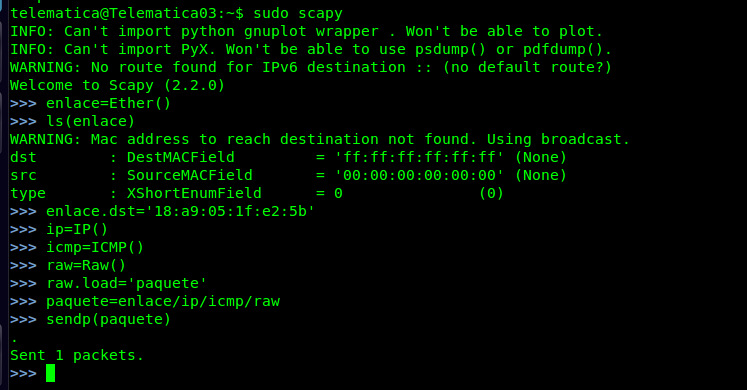
\includegraphics[scale=.37]{imagenes/Switch/Test_2.png}
\end{center}

Luego buscamos nuestro paquete en Wireshark para ver si se envio correctamente y llego a destino.

\begin{center}
	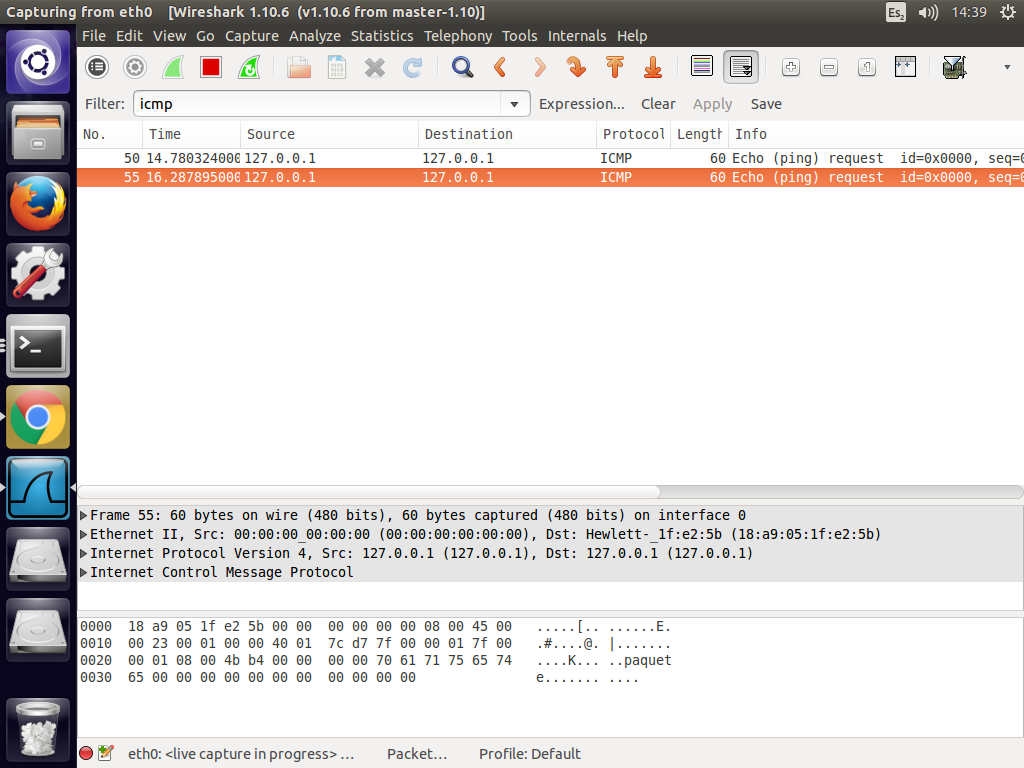
\includegraphics[scale=.37]{imagenes/Switch/Test_2_Wireshark.png}
\end{center}

\subsection{Envió de un paquete de datos con una MAC fuera de la red}

%agregar basura explicatoria, tengo paja y solo agregare las imagenes -Manuel

\begin{center}
	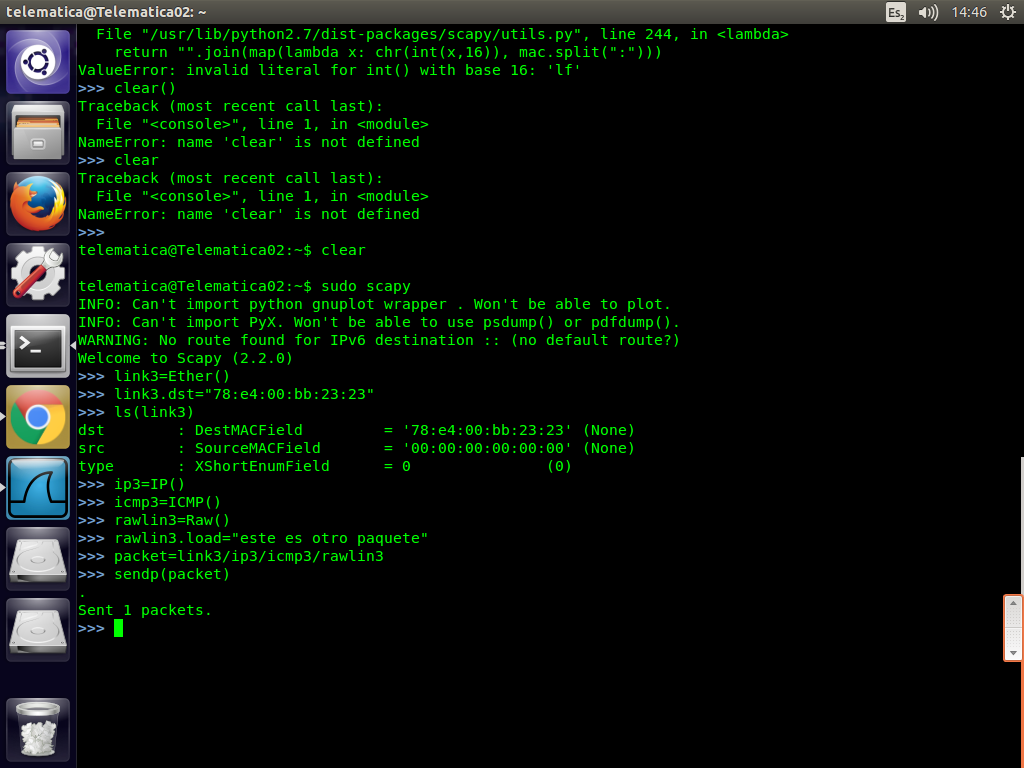
\includegraphics[scale=.37]{imagenes/Switch/Test_3.png}
\end{center}



\begin{center}
	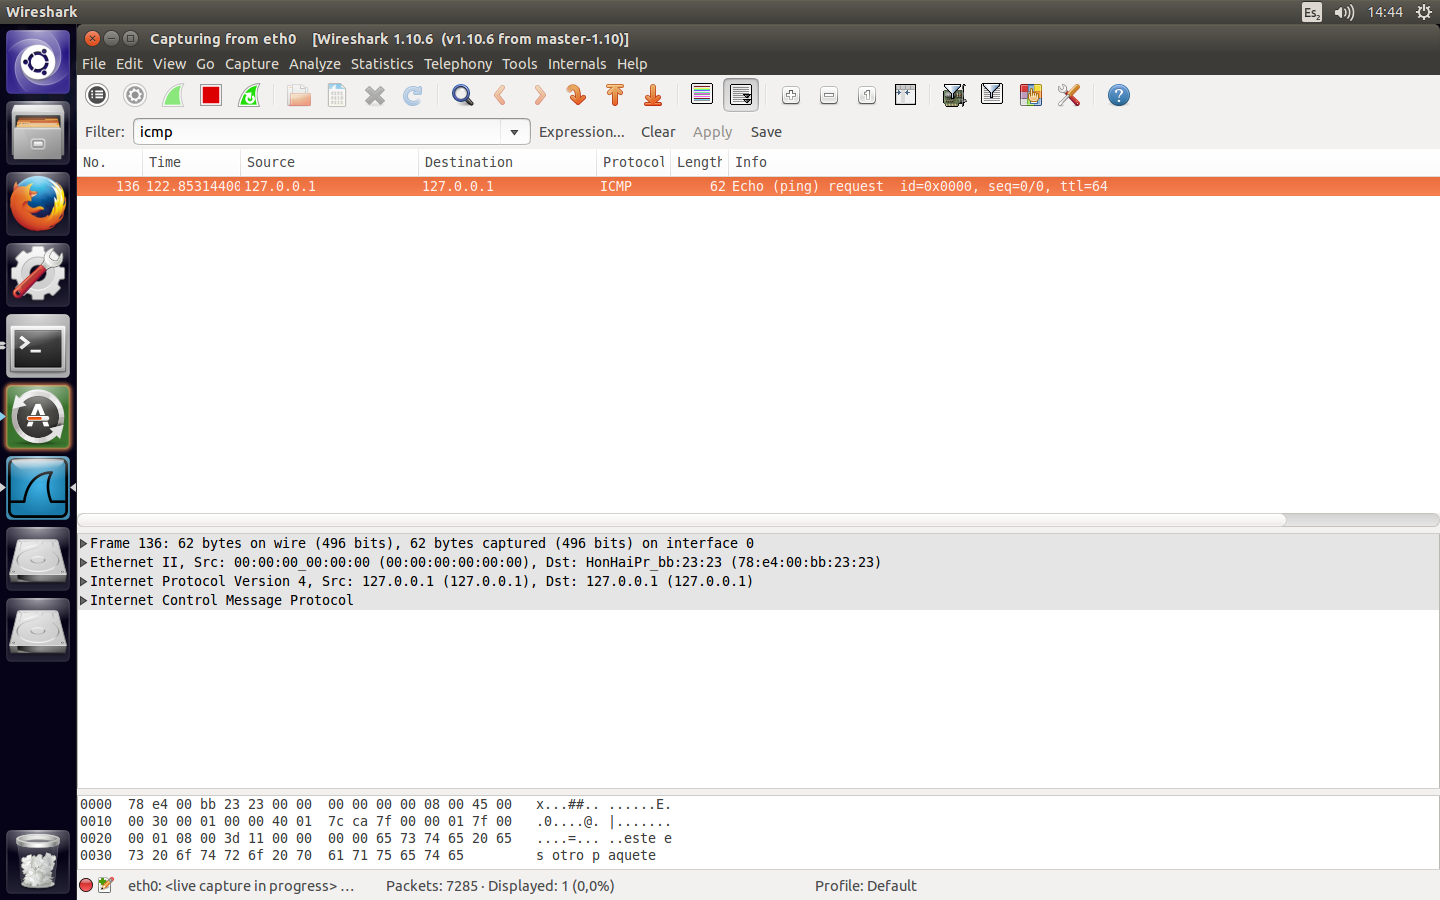
\includegraphics[scale=.37]{imagenes/Switch/Test_3_Wireshark.png}
\end{center}

\newpage

\section{Hub}

\subsection{Envío de un paquete de datos a FF:FF:FF:FF:FF:FF}

\subsection{Envío de un paquete de datos con MAC especifica}

\subsection{Envió de un paquete de datos con una MAC fuera de la red}

%Sigo pensando que es mejor que la dejemos en una seccion que consolide las deferencias entre HUB y Switch... - Manuel
% >Agregarlas en las secciones correspondientes -Manuel
%\section{Cuestionario}
%\subsection{¿Qué pasa cuando envió un paquete a la dirección 'FF:FF:FF:FF:FF:FF'?. ¿Quienes lo reciben?. ¿Por qué?}.

%\subsection{¿Qué pasa cuando envió un paquete a una MAC de otro equipo?. ¿Quieres lo pueden reciben?. ¿Por qué?.}

%\subsection{¿Qué sucede si envía un paquete a una MAC que no corresponda a ningún equipo de la red?. ¿Quienes lo pueden recepcionar?. ¿Por qué?.}

\chapter{Conclusión}

%A partir de la creación de paquetes de datos logramos comprender.....

\end{document}
